\documentclass[tikz,border=2mm]{standalone}
\usepackage{tikz}
\usetikzlibrary{shapes.geometric, arrows, shapes.gates.logic.US, calc}

\tikzstyle{arrow} = [thick,->,>=stealth]

\begin{document}
    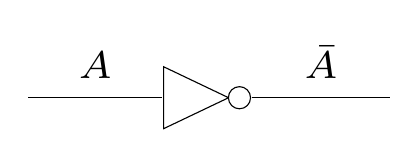
\begin{tikzpicture}[node distance=2cm, scale=2, every node/.style={scale=2}]
        
        \node at (1,0) [not gate US, logic gate inputs=nn,draw](not) {};
        
        \draw (not.output) -- node[above]{\scriptsize $\bar{A}$} (2.3, 0);
        \draw (0,0) -- node[above]{\scriptsize $A$} (not.input);
        
    \end{tikzpicture}
\end{document}
